\documentclass[10pt]{beamer}
%% beamer template and options 
\mode<presentation>
{
  \usetheme{CambridgeUS}
  \usefonttheme{serif}
  \useoutertheme{default}
}\setbeamertemplate{navigation symbols}{} 



\usepackage[utf8]{inputenc}
\usepackage{xcolor,comment,cancel}
\specialcomment{extended}{}{}    
\excludecomment{extended}
\usepackage{../styles/authordate1-4-beamer}

\usepackage{pgfplots}
\usepackage{xspace}
\usepackage{amsmath}
\usepackage{wasysym}
\usepackage{tikz}
\usetikzlibrary{automata,fit}
\usetikzlibrary{arrows}
\usetikzlibrary{shapes}
\usetikzlibrary{snakes}
\usetikzlibrary{arrows.meta,intersections}
\tikzstyle{every picture}+=[remember picture]
\usetikzlibrary{decorations.markings}





\title[IDL@BME-BIN] % (optional, use only with long paper titles)
{Introduction to Deep Learning} 
\subtitle{Multi-Layered NNet and the back-propagation algorithm}

\author[A. Allauzen] % (optional, use only with lots of authors)
{Alexandre Allauzen}



\institute[ESPCI/Dauphine/PSL] % (optional, but mostly needed)
{

\includegraphics[height=3em]{../logos/espci_blue.png}\hfill
\raisebox{1.75ex}{
\includegraphics[height=1.5em]{../logos/dauphine.png}}\\
\hfill
\includegraphics[height=3em]{../logos/logomiles_white.pdf}
}




\date{12/10/20} % (optional)





\DeclareMathOperator*{\argmax}{argmax}
\DeclareMathOperator*{\argmin}{argmin}

\newcommand{\ngram}{\mbox{$n$-gram}\xspace} 



%% important : red + bf 
\def\important#1{{\bf \color{red} #1\/}}


%%% basics : 
\newcommand{\real}{\ensuremath{\mathbb{R}}}
\newcommand{\vct}[1]{\ensuremath{\mathbf{#1}}} % a vector / matrix is in bold
\newcommand{\seq}[1]{\ensuremath{\boldsymbol{#1}}}

\newcommand{\transp}[1]{\ensuremath{{#1}^{t} }} % transposition 
%\newcommand{\scal}[2]{\left\langle #1 , #2 \right\rangle} % scalair
%product
\newcommand{\scal}[2]{#1^t#2} % scalair product
\newcommand{\mydot}[2]{\ensuremath{ \transp{#1} #2}} % dot prod
\newcommand{\norm}[1]{\ensuremath{|| #1 ||}} % l2
\newcommand{\normabs}[1]{\ensuremath{ || #1 ||_{1} }} % l1




% vertical vector 
\newcommand{\vv}[1]{
	\left(
	\begin{array}[c]{c}
		#1 
	\end{array}
	\right)
}
% backeted vertical vector 
\newcommand{\vvb}[1]{
	\left[
	\begin{array}[c]{c}
		#1 
	\end{array}
	\right]
}
% raw vertical vector 
\newcommand{\vvr}[1]{
	\begin{array}[c]{c}
		#1 
	\end{array}
}





% words sequences sentences 
\newcommand{\ws}{{w}} % 
\newcommand{\wseq}{{\mathbf{\ws}}} % 
\newcommand{\length}{{L}} % 
\newcommand{\wsseq}[2]{{\ws_{#1}^{#2}}} % word subsequence
\newcommand{\word}[1]{{\it #1}} % an example
\newcommand{\vocab}{{\mathcal{V}}} % vocab

\newcommand{\asymb}{\ensuremath{a}} % symbol of *one* element of the
                                % alignment sequence
\newcommand{\ssymb}{\ensuremath{s}} % symbol of *one* element of the source
\newcommand{\tsymb}{\ensuremath{t}} % symbol of *one* element of the target


\newcommand{\aseq}{\ensuremath{\mathbf{\asymb}}} % alignment sentence
\newcommand{\sseq}{\ensuremath{\mathbf{\ssymb}}} % source sentence
\newcommand{\tseq}{\ensuremath{\mathbf{\tsymb}}} % target sentence


% misc 
\newcommand{\BigO}[1]{\ensuremath{\operatorname{O}\bigl(#1\bigr)}}
\newcommand{\bos}{\texttt{\textless s\textgreater}} 
\newcommand{\eos}{\texttt{\textless/s\textgreater}} 


% machine learning i/o and parameters ...
% params for model 
\newcommand{\param}{\ensuremath{\theta}} 
\newcommand{\params}{\ensuremath{\boldsymbol{\theta}}}
\newcommand{\nfeats}{\ensuremath{D}} % 

\newcommand{\x}{\ensuremath{\seq{x}}} % 
\newcommand{\X}{\ensuremath{\seq{X}}} % 
\newcommand{\y}{\ensuremath{\seq{y}}} % 
\newcommand{\z}{\ensuremath{\seq{z}}} % 
\newcommand{\w}{\ensuremath{\seq{w}}} % 
\newcommand{\pa}{\ensuremath{\seq{a}}} % 
\newcommand{\pb}{\ensuremath{\seq{b}}} % 

\newcommand{\W}{\seq{W}}
\newcommand{\V}{\seq{V}}
\newcommand{\pgrad}[1]{\nabla_{#1}}
\newcommand{\vgrad}[2]{\ensuremath{\nabla_{#1} #2}}

%%%%%%% data and loss
\newcommand{\nsamples}{\ensuremath{N}}
\newcommand{\ploss}{\ensuremath{l}} % for one datapoint
\newcommand{\class}{\ensuremath{{c}}} %
\newcommand{\rvclass}{\ensuremath{{C}}} %  the class as a RV 
\newcommand{\sid}[1]{\ensuremath{_{(#1)}}} % sample id
\newcommand{\tid}[1]{_{(#1)}} % time index for parameters
\newcommand{\exi}{\ensuremath{\x\sid{i}}} % 
\newcommand{\classi}{\ensuremath{\class\sid{i}}} % 
\newcommand{\nclasses}{\ensuremath{C}} % 
\newcommand{\yi}{y\sid{i}}  % prediction for sample i 

\newcommand{\dataset}{\ensuremath{\mathcal{D}}} % training data
\newcommand{\datax}{\ensuremath{\mathcal{X}}} % training data, x part
\newcommand{\datay}{\ensuremath{\tilde{\mathcal{Y}}}} % training data y part  
\newcommand{\datac}{\ensuremath{\tilde{\mathcal{C}}}} % training data c part (classes)
\newcommand{\ty}{\ensuremath{\tilde{y}}} % the supervised answer
\newcommand{\fullloss}{\ensuremath{\mathcal{L}(\params;\dataset)}}

%%% 
\newcommand{\nlaw}{\mathcal{N}}
\newcommand{\bern}{\ensuremath{\pi}}



%%%%%%%%%%%%%%%%%%%%%%%%%%%%%%%%%%%%%%%%%%%%%%%%%%%%%%%%%%%%
% a vector as a grid 
% 1: x 
% 2: y
% 3: the number of cells 
% The template :
% \node[rectangle,rounded corners,  draw, fill=red!20, text width=0.3*\textwidth, minimum height=6ex]  (label) at (0,0) {Hello} ;
\newcommand{\xvector}[3]{%
  \draw[step=.25] (#1-0.001,#2) grid (#1+0.25,#2+#3*0.25 );%
}

% notations 
% a layer l 
% input x^{(l)}
% output y^{(l)}
%  y^{(l)} = f^{(l)}( W^{(l)} input)
% note that 
% y_i = W_i,: x
% W_ij : x_j -> y_i  
% k is for the class
% l for the layer 


%%%%%%% to define layers math notations 
\newcommand{\inp}{\ensuremath{\x}}
\newcommand{\outp}{\ensuremath{\seq{y}}}
\newcommand{\lid}[1]{\ensuremath{^{(#1)}}}

%%%%%%% data and loss
\newcommand{\dlta}{\ensuremath{\delta}} % gradient component of pre-activation
\newcommand{\vdlta}{\ensuremath{\seq{\delta}}} % gradient vector of pre-activation

\colorlet{darkgreen}{green!50!black}


%% draw one layer 
\newcommand{\layer}{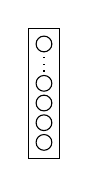
\begin{tikzpicture}[baseline=0.5ex]%
    \foreach \y in {0.25,0.5,...,1}{ 
      \draw (0,\y) circle  (0.1);%
    }
    \draw[dotted] (0.0, 1.15) -- (0.0,1.35); 
    \draw (0,1.5) circle (0.1);
    \draw (-0.2,0.05) rectangle (0.2,1.7);
\end{tikzpicture}}

%% draw connection
\newcommand{\connection}{\begin{tikzpicture}[baseline=0.5ex]%
    \draw[->] (0,0.85) -- (1.0,0.85);
\end{tikzpicture}}
%% dotted connection
\newcommand{\dotted}{\begin{tikzpicture}[baseline=0.5ex]%
    \draw[dotted,thick] (0,0.85) -- (0.5,0.85);%
\end{tikzpicture}}

\newcommand{\raiseW}{2ex}
% for computational graph
\newcommand{\vnode}{\node}
\newcommand{\funnode}{\node[minimum size=1.5,rectangle,draw=green,fill=green!20]}
\newcommand{\inlinefnode}[1]{\raisebox{-5pt}{\tikz{\funnode {#1}}}}



\newcommand{\justunder}{0.5cm}
\newcommand{\largeurUn}{0.8}
\newcommand{\largeurDeux}{0.7}
\setbeamercolor{postit}{fg=black,bg=red!30}
\setbeamercolor{mygreen}{fg=black,bg=green!20}
\setbeamercolor{myred}{fg=black,bg=red!20}
\setbeamercolor{darkpostit}{fg=black,bg=red!64}
\setbeamercolor{text}{fg=black,bg=red!10}


%%%%%%%%%% NNet for NLP
%% draw one layer  
\newcommand{\wemb}{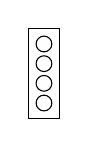
\begin{tikzpicture}[baseline=0.5ex]%
    \foreach \y in {0.25,0.5,...,1}{ 
      \draw (0,\y) circle  (0.1);%
    }
    \draw (-0.2,0.05) rectangle (0.2,1.2);
\end{tikzpicture}}

\newcommand{\worddim}{\ensuremath{K}} % dimension of the word embeddings
\newcommand{\wvector}{\ensuremath{\vct{v}}} % word vector
\newcommand{\wmatrix}{\ensuremath{\vct{R}}} % word matrix
\newcommand{\dvector}{\ensuremath{\vct{d}}} % document vector



%%%%%%%%% macro et redefinition 
\AtBeginSection[]
{
  \begin{frame}<beamer>
    \frametitle{Outline}
    \tableofcontents[currentsection]
  \end{frame}
}


\begin{document}
\tikzset{->-/.style={decoration={
  markings,
  mark=at position .5 with {\arrow{>}}},postaction={decorate}}}

\begin{frame}
  \titlepage
\end{frame}

\begin{frame}<beamer>
  \frametitle{Outline}
  \tableofcontents
\end{frame}
 


%%%%%%%%%%%%%%%%%%%%%%%%%%%%%%%%%%%%%%%%%%%%%%%%%%%%%%%%%%%%%%%%%%%%%%
\section{From logistic regression to neural network}
% - Multi-class classification
% From binary to multi-class / Regression : architecture and loss function
% see https://machinelearningmastery.com/how-to-choose-loss-functions-when-training-deep-learning-neural-networks/
% - Matrix operation
% Mini-batch operation 
%%%%%%%%%%%%%%%%%%%%%%%%%%%%%%%%%%%%%%%%%%%%%%%%%%%%%%%%%%%%%%%%%%%%%%%%%%%%%%%%%%%%%%%%%
\begin{frame}
  \frametitle{A choice of terminology}
  % logistic regression
  \begin{block}{Logistic regression (binary classification)}
    \begin{columns}
      %%%%%%%%%%%%%%%%%%%%%%%%%%%%%%%%% 
      % dot product + function 
      \begin{column}{0.4\textwidth}
        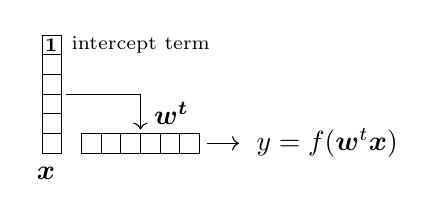
\begin{tikzpicture}
          \only<1->{
            % x
            \draw[step=.25] (0,-0) grid (0.25, 1.5);%
            \node (x) at (0.05,-0.25) {$\x$};%
            \node (bias) at (0.115,1.37) {\scriptsize{\textbf{1}}};
            \node[anchor=west] (bias2) at (0.25,1.37) {\scriptsize{intercept term}};
            
            % w^t
            \draw[step=.25] (0.49,0) grid (2.0, 0.25);%
            \node[anchor=west] (w) at (1.3,0.5) {$\seq{w^t}$};%
            \draw (0.3,0.75) -- (1.25,0.75);%
            \draw[->] (1.25,0.75) -- (1.25,0.3);%
            % res 1
            \draw[->] (2.1,0.125) -- (2.5,0.125);%
            \node[anchor=west] (y) at (2.6,0.125) {$y =
              f( \scal{ \seq{w}}{\x})$};%
          }
        \end{tikzpicture}
        $$ 
        f(a=\scal{\seq{w}}{\x}) = \frac{e^{a}}{1+e^{a}} = \sigma(a)
        $$
      \end{column}
      % the logistic regression
      \begin{column}{0.6\textwidth}
        \begin{center}
          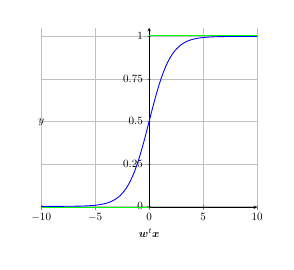
\begin{tikzpicture}[scale=0.4]
            \begin{axis}%
              [ %%%%%%%%%%%%%%%%%
              grid=major, %
              xmin=-10, % 
              xmax=10, % 
              axis x line=bottom, % 
              ytick={0,.25,.5,.75,1.0}, %
              ymax=1.05, % 
              axis y line=middle, % 
              xlabel = $\scal{\seq{w}}{\x}$, %
              ylabel = $y$, % 
              every  axis y label/.style={at={(current axis.north  west)},above=2mm} ]% 
              %%%%%%%%% binary classif in green
              \addplot%
              [ blue,thick,%
              mark=none, samples=100, domain=-10:10, ]
              (x,{1/(1+exp(-x))});
              \addplot%
              [ green,very thick,%
              mark=none, samples=100, domain=0:10, ]
              (x,{1.005});
              \addplot%
              [ green,very thick,%
              mark=none, samples=100, domain=-10:0, ]
              (x,{-0.005});
            \end{axis}
          \end{tikzpicture}
        \end{center}
      \end{column}
    \end{columns}
  \end{block}
  %%%%%%%% neuronal view 
  \pause
  \begin{block}{A single artificial neuron}
    \begin{columns}
      %%%%%%%%%%%%%%%%%%% left 
      \begin{column}{0.4\textwidth}
        \begin{tikzpicture}
          % neurone 1
          \draw[red] (1,1) circle (0.1cm);% output 1
          \node[anchor=west] (ny1) at (1.5,1){{\color{red}{ $y=f( \scal{\seq{w}}{\x})$}}};
          % input
          \node (nx) at (-0.75,0.625){$\x$}; %
          \draw[snake=brace] (-0.45,-0.125) -- (-0.45,1.375); 
          \node (bias) at (-0.25,1.25){\scriptsize{\textbf{1}}}; %
          \node[anchor=west] (bias2) at (-0.25,1.5){\scriptsize{bias term}}; %
          % draw neurons
          \node[color=red] (nw) at (0.55,0.1){$\seq{w}$}; %
          \foreach \y in {0,0.25,...,1.25}{ \draw (0,\y) circle (0.1cm);%
            \draw[->-,red] (0.125,\y) -- (0.875,1); }
          \draw[fill=black] (0,1.25) circle (0.1cm);% bias neuron
        \end{tikzpicture}
      \end{column}
      %%%%%%%%%%%%%%%%%%% right
      \begin{column}{0.6\textwidth}
        \begin{itemize}
        \item pre-activation : $a= \scal{\seq{w}}{\x}$
        \item $f$: activation function 
        \item Input values =  input ``neurones''
        \item $\x$: a vector of values, a layer
        \end{itemize}
      \end{column}
    \end{columns}
  \end{block}
\end{frame}



%%%%%%%%%%%%%%%%%%%%%%%%%%%%%%%%%%%%%%%%%%%%%%%%% 
\begin{frame}{A choice of terminology - 2}
  \begin{block}{From binary classification to $\nclasses$ classes (Maxent)}
    \begin{columns}
      %%%%%%%%%%%%%%%%%%%%%%%%%%%%%%%%% 
      % dot product + function 
      \begin{column}{0.5\textwidth}
        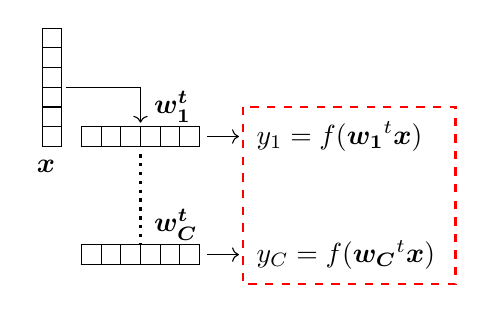
\begin{tikzpicture}
          {
            % x
            \draw[step=.25] (0,-0) grid (0.25, 1.5);%
            \node (x) at (0.05,-0.25) {$\x$};%
            
            % w^t
            \draw[step=.25] (0.49,0) grid (2.0, 0.25);%
            \node[anchor=west] (w) at (1.3,0.5) {$\seq{w_1^t}$};%
            \draw (0.3,0.75) -- (1.25,0.75);%
            \draw[->] (1.25,0.75) -- (1.25,0.3);%
            % res 1
            \draw[->] (2.1,0.125) -- (2.5,0.125);%
            \node[anchor=west] (y) at (2.6,0.125) {$y_1 =
              f( \scal{ \seq{w_1}}{\x})$};%
          }
          {
            % res k
            \draw[dotted, very thick] (1.25,-0.1) -- (1.25,-1.25);%
            \begin{scope}[yshift=-1.5cm]
              \draw[step=.25] (0.49,0) grid (2.0, 0.25);%
              \node[anchor=west] (wk) at (1.3,0.5) {$\seq{w_{\nclasses}^t}$};%
              \draw[->] (2.1,0.125) -- (2.5,0.125);%
              \node[anchor=west] (y) at (2.6,0.125) {$y_{\nclasses} =
                f(\scal{\seq{w_{\nclasses}}}{\x})$};%
            \end{scope}
          }
          {% square together the output
            \draw[red,dashed,thick] (2.55, 0.5) rectangle (5.25,-1.75);
          }
        \end{tikzpicture}
      \end{column}
      % the maxent function
      \begin{column}{0.5\textwidth}
        \begin{align*}
          y_k &= f(a_k=\scal{\seq{w_k}}{\x})= P(c=k|\x)\\
              &= \frac{e^{a_k}}{\color{red}\sum_{k'=1}^{\nclasses} e^{a_{k'}}}= \frac{e^{a_k}}{\color{red}Z(\x)} \\
          \sum_{k=1}^{\nclasses} y_k &= \sum_{k=1}^{\nclasses}P(c=k|\x) =1 
        \end{align*}
      \end{column}
    \end{columns}
  \end{block}
  %%%%%%%% neuronal view 
  \pause
  \begin{block}{A simple neural network}
    \begin{columns}
      \begin{column}{0.5\textwidth}
        \begin{tikzpicture}
          % neurone 1
          \draw[red] (1,1) circle (0.1cm);% output 1
          \node[anchor=west,red] (ny1) at (1.5,1){$y_1=
            f(\seq{w_1^t}\x)$}; %
          % input
          \node (nx) at (-0.5,0.625){$\x$}; %
          \node[color=red] (nw) at (0.5,1.4){$\seq{w_1}$}; %
          \foreach \y in {0,0.25,...,1.25}{ \draw (0,\y) circle
            (0.1cm);%
            \draw[->-,red] (0.125,\y) -- (0.875,1); }
          
          \draw[snake=brace] (-0.2,-0.125) -- (-0.2,1.375);

          % neurone {\nclasses}
          
          \foreach \a in {0.75}{ \draw[green] (1,1-\a) circle
            (0.1cm);% output 2
            \node[color=green] (nw2) at (0.5,-0.25){ $\seq{w_{\nclasses}}$}; %
            \node[anchor=west,green] (ny2) at (1.5,1-\a){$y_{\nclasses}=
              f(\seq{w_{\nclasses}^t}\x)$}; %

            \foreach \y in {0,0.25,...,1.25}{ \draw[->-,green]
              (0.125,\y) -- (0.875,1-\a); }
            % dotted between output neurones:
            \draw[dotted,very thick] (1,0.9) -- (1,0.35);

          }
        \end{tikzpicture}
        % 
      \end{column}
      \begin{column}{0.5\textwidth}
        \begin{itemize}
        \item $\x$: \emph{input layer}
        \item $\seq{y}$: \emph{output layer}
        \item each $y_k$ has its parameters $\seq{w}_k$
        \item $f$ is the \important{softmax} function
        \end{itemize}
      \end{column}
    \end{columns}
  \end{block}
\end{frame}

%%%%%%%%%%%%%%%%%%%%%%%%%%%%%%%%%%%%%%%%%%%%%%%%%%%%%%%%%%%%%%%%%%%%%%%%%%%%%%% 
\begin{frame}
  \frametitle{Two layers fully connected}
  \begin{center}
    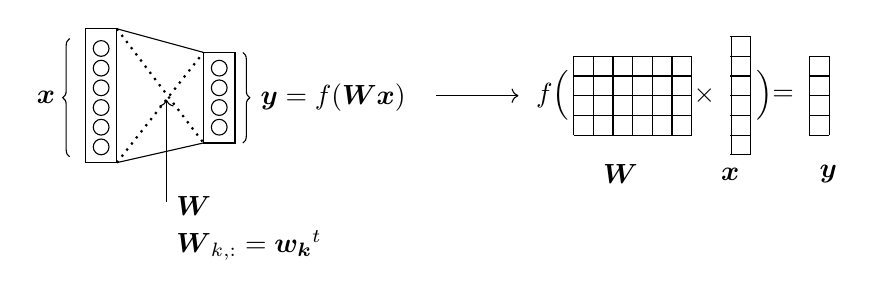
\begin{tikzpicture}
      \begin{scope}
        % input
        \node (nx) at (-0.7,0.625){$\x$}; %
        \foreach \y in {0,0.25,...,1.25}{ 
          \draw (0,\y) circle  (0.1cm);%
        }
        \draw (-0.2,-0.2) rectangle (0.2,1.5);
        \draw[snake=brace] (-0.4,-0.125) -- (-0.4,1.375); 
        % output
        \foreach \y in {0.25,0.5,...,1}{ 
          \draw (1.5,\y) circle  (0.1cm);%
        }
        \draw (1.3,0.05) rectangle (1.7,1.2);
        \draw (0.2,-0.2) -- (1.3,0.05); 
        \draw (0.2,1.5) -- (1.3,1.2);
        \draw[dotted, thick] (0.2,1.5) -- (1.3,0.05);
        \draw[dotted,thick] (0.2,-0.2) -- (1.3,1.2); 
        \draw[snake=brace] ( 1.8, 1.2) --(1.8, 0.05) ; 
        \node[anchor=west] (ny) at (1.9,0.625){$\seq{y}=f(\W \x)$}; %
        \node[anchor=west] (nW) at (0.83,-0.75){$\W$};%
        \node[anchor=west] (nW) at (0.83,-1.25) {$\W_{k,:}=\seq{w_k}^t$}; %
        \draw[->]  (0.83,-0.7) -- (0.83,0.6);%
      \end{scope}
      %%%%%%%%%%%%%%%%%%%%%%%%%%%%%%%%%%%%%%%%%% 
      %% matrix view 
      %%%%%%%%%%%%%%%%%%%%%%%%%%%%%%%%%%%%%%%%%% 
      \only<2->{
        \begin{scope}[xshift=6cm,yshift=0.15cm]
          
          \draw[->] (-1.75,0.5) -- (-0.7,0.5);
          \draw[step=.25] (0,-0) grid (1.5, 1);%
          \draw[step=.25] (1.99,-0.25) grid (2.25, 1.25 );%
          \draw[step=.25] (2.99,-0) grid (3.25, 1 );%
          % oper
          \node[anchor=west] (times) at (1.4, 0.5) {$\times$};
          \node[anchor=west] (equals) at (2.4, 0.5) {$=$};
          % names
          \node[anchor=west] (f) at (-0.6, 0.5) {$f\Big($};
          \node[anchor=west] (fe) at (2.2, 0.5) {$\Big)$};
          \node[anchor=west] (W) at (0.25, -0.5) {$\seq{W}$};
          \node[anchor=west] (x) at (1.75, -0.5) {$\seq{x}$};
          \node[anchor=west] (x) at (3, -0.5) {$\seq{y}$};
        \end{scope}
      }
    \end{tikzpicture}
  \end{center}
  \pause\pause
  {
    \begin{columns}
      \column{0.5\textwidth}
      Activation $f$:
      \begin{itemize}
      \item $f$ is usually a non-linear function
      \item $f$ is a component wise function
      \item tanh, sigmoid, relu, ...
      \end{itemize}
      \column{0.5\textwidth}
      Dimensions: 
      \begin{itemize}
      \item $\x: \nfeats \times 1 $
      \item $\seq{W}: \nclasses \times \nfeats $
      \item $\seq{y}: (\nclasses \times \xcancel{ \nfeats) \times (  \nfeats }
        \times 1 ) =\nclasses \times 1 $
      \end{itemize}
    \end{columns}
    \textit{e.g} the softmax function:
    $$      
    y_k = P(c=k|\x) = \frac{e^{\scal{\seq{w_k}}{\x}} }{\sum_{k'}e^{\scal{\seq{w_{k'}}}{\x}}}
    = \frac{e^{\W_{k,:}\x}}{\sum_{k'} e^{\W_{k',:}\x}}
    $$   
  }
\end{frame}



%%%%%%%%%%%%%%%%%%%%%%%%%%%%%%%%%%%%%%%%%%%%%%%%%%%%%%%%%%%%%%%%%%%%%%%%%%%%%%% 
%%%%%%%% use the cancel package 
\begin{frame}{Matrix and Vector product}
  \begin{center}
    \begin{tabular}{rllr}
      $ \vct{y}$ &\ $=\ \W$ &$\ \times\ \x$ \\[2ex]
      %%%%%%%% line with figs 
      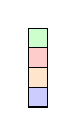
\begin{tikzpicture}

        \draw[fill=green!20] (0,0.5) rectangle (0.25, 0.25);
        \draw[fill=red!20] (0,0.25) rectangle (0.25, 0.0);
        \draw[fill=orange!20] (0,0.0) rectangle (0.25, -0.25);
        \draw[fill=blue!20] (0,-0.25) rectangle (0.25, -0.5);
        \draw[step=.25] (0,-0.5) grid (0.25, 0.5);
      \end{tikzpicture}
      
                &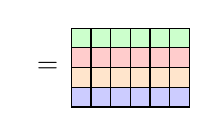
\begin{tikzpicture}
                          \node at (-0.3,-0) {$=$};
        \draw[fill=green!20] (0,0.5) rectangle (1.5, 0.25);
        \draw[fill=red!20] (0,0.25) rectangle (1.5, 0.0);
        \draw[fill=orange!20] (0,0.0) rectangle (1.5, -0.25);
        \draw[fill=blue!20] (0,-0.25) rectangle (1.5, -0.5);
        \draw[step=.25] (0,-0.5) grid (1.5, 0.5);
      \end{tikzpicture}

      &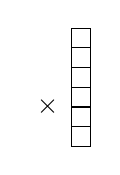
\begin{tikzpicture}
        \node at (-0.3,-0.25) {$\times$};
        \draw[step=.25] (0,-0.75) grid (0.25, 0.75);
      \end{tikzpicture}\\[2ex]
      %%%%%
      \color{green!60}$y_1$ &\color{green}$\ =\ \W_{1,:}$ &$\  \times\ \x$\\
      \color{red!60}$y_2$ &\color{red!60}$\ =\ \W_{2,:}$ &$\  \times\ \x$\\
      \ $\cdots$ &\ $\cdots$ &$\ \cdots$
    \end{tabular}
\end{center}
In terms of dimension: 
\begin{displaymath}
  \textrm{With } \left\{
    \begin{array}{ll}
      \x  &: (L_1 \times 1)\\
      \W  &: (L_2 \times C_2)\\
      \seq{y} &: (L_2 \times 1)
    \end{array} \right. \Rightarrow (\W\x) :
   (L_2 \times 1)= (L_2 \times \underbrace{\xcancel{C_2) (L_1 } }_{\color{red}C_2=L_1} \times 1)
\end{displaymath}
\end{frame}

%%%%%%%%%%%%%%%%%%%%%%%%%%%%%%%%%%%%%%%%%%%%%%%%%%%%%%%%%%%%%%%%%%%%%%%%%%%%%%% 
%%%%%%%% use the cancel package 
\begin{frame}{Matrix-matrix product}
  $\seq{X}$ is a matrix of 2 columns, 2 vectors as $\x$: 
  \begin{center}
    \begin{tabular}{rllr}
      $ \seq{Y}$ &\ $=\W$ &$\ \times\ \seq{X}$ \\[2ex]
      %%%%%%%% line with figs 
      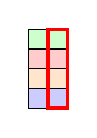
\begin{tikzpicture}
        % matrix Y 
        \draw[fill=green!20] (0,0.5) rectangle (0.5, 0.25);
        \draw[fill=red!20] (0,0.25) rectangle (0.5, 0.0);
        \draw[fill=orange!20] (0,0.0) rectangle (0.5, -0.25);
        \draw[fill=blue!20] (0,-0.25) rectangle (0.5, -0.5);
        \draw[step=.25] (0,-0.5) grid (0.5, 0.5);
        \draw[draw=red,very thick] (0.25,-0.5) rectangle (0.5, 0.5);
      \end{tikzpicture}
      % matrix W
                &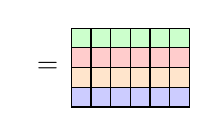
\begin{tikzpicture}
                          \node at (-0.3,-0) {$=$};
        \draw[fill=green!20] (0,0.5) rectangle (1.5, 0.25);
        \draw[fill=red!20] (0,0.25) rectangle (1.5, 0.0);
        \draw[fill=orange!20] (0,0.0) rectangle (1.5, -0.25);
        \draw[fill=blue!20] (0,-0.25) rectangle (1.5, -0.5);
        \draw[step=.25] (0,-0.5) grid (1.5, 0.5);
      \end{tikzpicture}
      % Matrix X 
      &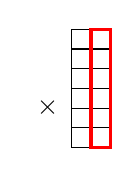
\begin{tikzpicture}
        \node at (-0.3,-0.25) {$\times$};
        \draw[step=.25] (0,-0.75) grid (0.5, 0.75);
        \draw[draw=red,very thick] (0.25,-0.75) rectangle (0.5, 0.75);
      \end{tikzpicture}
      %%%%%
    \end{tabular}
\end{center}
In terms of dimension: 
\begin{displaymath}
  \textrm{With } \left\{
    \begin{array}{ll}
      \seq{X}  &: (L_1 \times C_1)\\
      \W  &: (L_2 \times C_2)\\
      \seq{y} &: (L_2 \times C_1)
    \end{array} \right. \rightarrow
   (L_2 \times C_2)= (L_2 \times \underbrace{\xcancel{C_2) (L_1 } }_{\color{red}C_2=L_1} \times C_1)
\end{displaymath}
\end{frame}



%%%%%%%%%%%%%%%%%%%%%%%%%%%%%%%%%%%%%%%%%%%%%%%%%%%%%%%%%%%%%%%%%%%%%%%%%%%%%%% 
\begin{frame}{Bias or not bias}
  \begin{block}{Implicit Bias}
    \begin{center}
      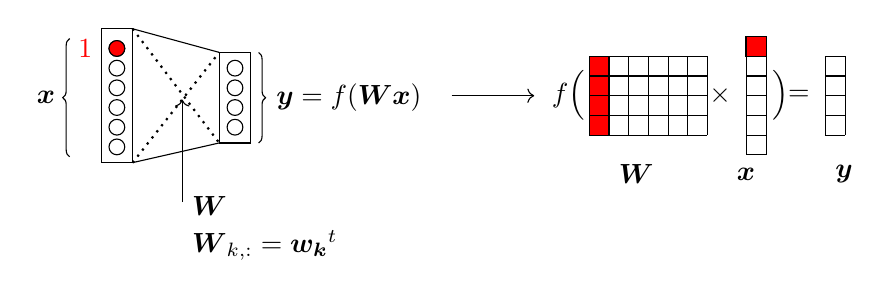
\begin{tikzpicture}
        \begin{scope}
          % input

        \node (nx) at (-0.9,0.625){$\x$}; %
        \draw[snake=brace] (-0.6,-0.125) -- (-0.6,1.375); 

        \foreach \y in {0,0.25,...,1.25}{ 
          \draw (0,\y) circle  (0.1cm);%
        }
        \draw (-0.2,-0.2) rectangle (0.2,1.5);        
        % the first node is a constant set to one 
        \draw[fill=red] (0,1.25) circle  (0.1cm);%
        \node[red] (nx) at (-0.4,1.25){$1$}; %
        
        

        % output
        \foreach \y in {0.25,0.5,...,1}{ 
          \draw (1.5,\y) circle  (0.1cm);%
        }
        \draw (1.3,0.05) rectangle (1.7,1.2);
        \draw (0.2,-0.2) -- (1.3,0.05); 
        \draw (0.2,1.5) -- (1.3,1.2);
        \draw[dotted, thick] (0.2,1.5) -- (1.3,0.05);
        \draw[dotted,thick] (0.2,-0.2) -- (1.3,1.2); 
        \draw[snake=brace] ( 1.8, 1.2) --(1.8, 0.05) ; 
        \node[anchor=west] (ny) at (1.9,0.625){$\seq{y}=f(\W \x)$}; %
        \node[anchor=west] (nW) at (0.83,-0.75){$\W$};%
        \node[anchor=west] (nW) at (0.83,-1.25) {$\W_{k,:}=\seq{w_k}^t$}; %
        \draw[->]  (0.83,-0.7) -- (0.83,0.6);%
      \end{scope}
      %%%%%%%%%%%%%%%%%%%%%%%%%%%%%%%%%%%%%%%%%% 
      %% matrix view 
      %%%%%%%%%%%%%%%%%%%%%%%%%%%%%%%%%%%%%%%%%% 
        \begin{scope}[xshift=6cm,yshift=0.15cm]

          % bias term in x 
          \draw[fill=red] (1.99,1) rectangle (2.25, 1.25 );%
          % bias term in W 
          \draw[fill=red] (0,-0) rectangle (0.25, 1);%
          % grids for matrix and vectors
          \draw[->] (-1.75,0.5) -- (-0.7,0.5);
          \draw[step=.25] (0,-0) grid (1.5, 1);%
          \draw[step=.25] (1.99,-0.25) grid (2.25, 1.25 );%
          \draw[step=.25] (2.99,-0) grid (3.25, 1 );%
          % oper
          \node[anchor=west] (times) at (1.4, 0.5) {$\times$};
          \node[anchor=west] (equals) at (2.4, 0.5) {$=$};
          % names
          \node[anchor=west] (f) at (-0.6, 0.5) {$f\Big($};
          \node[anchor=west] (fe) at (2.2, 0.5) {$\Big)$};
          \node[anchor=west] (W) at (0.25, -0.5) {$\seq{W}$};
          \node[anchor=west] (x) at (1.75, -0.5) {$\seq{x}$};
          \node[anchor=west] (x) at (3, -0.5) {$\seq{y}$};
        \end{scope}
    \end{tikzpicture}
  \end{center}
  \end{block}

  \begin{block}{Explicit bias}
    \begin{center}
      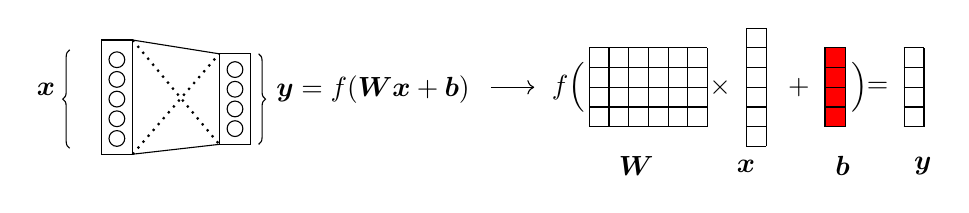
\begin{tikzpicture}
        \begin{scope}
          % input

        \node (nx) at (-0.9,0.625){$\x$}; %
        \draw[snake=brace] (-0.6,-0.125) -- (-0.6,1.125); 

        \foreach \y in {0,0.25,...,1}{ 
          \draw (0,\y) circle  (0.1cm);%
        }
        \draw (-0.2,-0.2) rectangle (0.2,1.25);        

        % output
        \foreach \y in {0.25,0.5,...,1}{ 
          \draw (1.5,\y-0.125) circle  (0.1cm);%
        }
        \draw (1.3,0.05-0.125) rectangle (1.7,1.2-0.125);
        \draw (0.2,-0.2) -- (1.3,0.05-0.125); 
        \draw (0.2,1.25) -- (1.3,1.2-0.125);
        \draw[dotted, thick] (0.2,1.25) -- (1.3,0.05-0.125);
        \draw[dotted,thick] (0.2,-0.2) -- (1.3,1.2-0.125); 
        \draw[snake=brace] ( 1.8, 1.2-0.125) --(1.8, 0.05-0.125) ; 
        \node[anchor=west] (ny) at (1.9,0.625){$\seq{y}=f(\W \x + \seq{b})$}; %
      \end{scope}
      %%%%%%%%%%%%%%%%%%%%%%%%%%%%%%%%%%%%%%%%%% 
      %% matrix view 
      %%%%%%%%%%%%%%%%%%%%%%%%%%%%%%%%%%%%%%%%%% 
        \begin{scope}[xshift=6cm,yshift=0.15cm]
          \draw[->] (-1.25,0.5) -- (-0.7,0.5);

          \draw[fill=red] (2.99,-0) rectangle (3.25, 1 );% bias in red
          % grids for matrix and vectors
          \draw[step=.25] (0,-0) grid (1.5, 1);% W 
          \draw[step=.25] (1.99,-0.25) grid (2.25, 1.25 );% x
          \draw[step=.25] (2.99,-0) grid (3.25, 1 );% b
          \draw[step=.25] (3.99,-0) grid (4.25, 1 );% y 
          % oper
          \node[anchor=west] (times) at (1.4, 0.5) {$\times$};
          \node[anchor=west] (equals) at (2.4, 0.5) {$+$};
          \node[anchor=west] (equals) at (3.4, 0.5) {$=$};
          % names
          \node[anchor=west] (f) at (-0.6, 0.5) {$f\Big($};
          \node[anchor=west] (fe) at (3.2, 0.5) {$\Big)$};
          \node[anchor=west] (W) at (0.25, -0.5) {$\seq{W}$};
          \node[anchor=west] (x) at (1.75, -0.5) {$\seq{x}$};
          \node[anchor=west] (x) at (3, -0.5) {$\seq{b}$};
          \node[anchor=west] (x) at (4, -0.5) {$\seq{y}$};
        \end{scope}
    \end{tikzpicture}
  \end{center}

  \end{block}
\end{frame}


%%%%%%%%%%%%%%%%%%%%%%%%%%%%%%%%%%%%%%%%%%%%%%%%%%%%%%%%%%%%%%%%%%%%%%%%
\begin{frame}{Classification with a simple neural network}
  \begin{block}{Binary classification}
    \begin{itemize}
    \item The input layer is a vector ($\x$), it encodes the data
    \item A single output neuron transform $\x$,  $\seq{w}$ are its parameters
    \item With a sigmoïd activation, the loss function is the binary cross entropy, the log-loss,
      minus the log-likelihood, ...
    \end{itemize}
  \end{block}
  \begin{block}{Multiclass}
    \begin{itemize}
    \item The input layer is a vector ($\x$) 
    \item The output layer $\y$ contains one neuron per class  
    \item It transforms $\x$, $\W$ are the parameters of the output layer
    \item $\W$ gathers the $\seq{w}_k= \W_{k,:}$
    \item With a softmax activation, the loss function is the cross entropy, the log-loss,
      minus the log-likelihood, ...
    \end{itemize}
  \end{block}
  \begin{center}
    {\color{red} Other loss functions exist for classification}
  \end{center}
\end{frame}

%%%%%%%%%%%%%%%%%%%%%%%%%%%%%%%%%%%%%%%%%%%%%%%%%%%%%%%%%%%%%%%%%%%%%%%%
\begin{frame}{Regression with a simple neural network}
  \begin{block}{Simple linear regression}
    $$
    y = f_{\params} (\x),\  y\in\real
    $$
    \begin{itemize}
    \item The input layer is a vector ($\x$), it encodes the data
    \item A single output neuron for $y$ ($\seq{w}$ are its parameters)
    \item The activation function depends on the output domain
    \end{itemize}
  \end{block}
  \begin{block}{Multi-variate linear regression}
    $$
    \y = f_{\params} (\x),\  \y\in\real^{\nclasses}
    $$
    \begin{itemize}
    \item The input layer is a vector ($\x$) 
    \item The output layer $\y$ contains one neuron per output value
    \item It transforms $\x$ in $\y$, $\W$ are the parameters of the output layer
    \end{itemize}
  \end{block}
\end{frame}


%%%%%%%%%%%%%%%%%%%%%%%%%%%%%%%%%%%%%%%%%%%%%%%%%%%%%%%%%%%%%%%%%%%%%%%%
\begin{frame}{Loss for regression}
  \framesubtitle{The Mean Squarred Error \textit{a.k.a} MSE}
  \begin{align*}
\dataset &= (\exi, \y\sid{i})_{i=1}^{\nsamples}, \\
\fullloss &= \frac{1}{\nsamples} \sum_{i=1}^{\nsamples} ||\y\sid{i} - f_{\params}(\exi) ||^2
  \end{align*}
  \begin{center}
    \includegraphics[width=0.6\textwidth]{./figs/mse}
  \end{center}
  \begin{center}
    {\color{red} Other loss functions exist for regression}
  \end{center}

\end{frame}

%%%%%%%%%%%%%%%%%%%%%%%%%%%%%%%%%%%%%%%%%%%%%%%%%%%%%%%%%%%%%%%%%%%%%%%%
\begin{frame}
  \frametitle{Two layers fully connected: another view}
  \begin{center}
    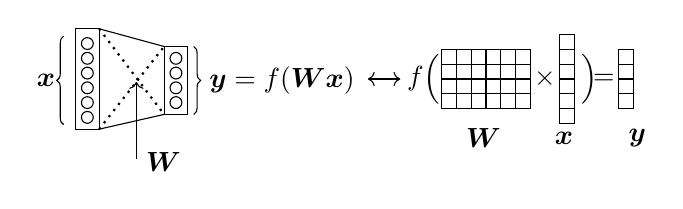
\begin{tikzpicture}[scale=0.75]
      \begin{scope}
        % input
        \node (nx) at (-0.7,0.625){$\x$}; %
        \foreach \y in {0,0.25,...,1.25}{ 
          \draw (0,\y) circle  (0.1cm);%
        }
        \draw (-0.2,-0.2) rectangle (0.2,1.5);
        \draw[snake=brace] (-0.4,-0.125) -- (-0.4,1.375); 
        % output
        \foreach \y in {0.25,0.5,...,1}{ 
          \draw (1.5,\y) circle  (0.1cm);%
        }
        \draw (1.3,0.05) rectangle (1.7,1.2);
        \draw (0.2,-0.2) -- (1.3,0.05); 
        \draw (0.2,1.5) -- (1.3,1.2);
        \draw[dotted, thick] (0.2,1.5) -- (1.3,0.05);
        \draw[dotted,thick] (0.2,-0.2) -- (1.3,1.2); 
        \draw[snake=brace] ( 1.8, 1.2) --(1.8, 0.05) ; 
        \node[anchor=west] (ny) at (1.9,0.625){$\seq{y}=f(\W \x)$}; %
        \node[anchor=west] (nW) at (0.83,-0.75){$\W$};%
        \draw[->]  (0.83,-0.7) -- (0.83,0.6);%
      \end{scope}
      %%%%%%%%%%%%%%%%%%%%%%%%%%%%%%%%%%%%%%%%%% 
      %% matrix view 
      %%%%%%%%%%%%%%%%%%%%%%%%%%%%%%%%%%%%%%%%%% 
        \begin{scope}[xshift=6cm,yshift=0.15cm]
          
          \draw[<->] (-1.25,0.5) -- (-0.7,0.5);
          \draw[step=.25] (0,-0) grid (1.5, 1);%
          \draw[step=.25] (1.99,-0.25) grid (2.25, 1.25 );%
          \draw[step=.25] (2.99,-0) grid (3.25, 1 );%
          % oper
          \node[anchor=west] (times) at (1.4, 0.5) {$\times$};
          \node[anchor=west] (equals) at (2.4, 0.5) {$=$};
          % names
          \node[anchor=west] (f) at (-0.75, 0.5) {$f\Big($};
          \node[anchor=west] (fe) at (2.2, 0.5) {$\Big)$};
          \node[anchor=west] (W) at (0.25, -0.5) {$\seq{W}$};
          \node[anchor=west] (x) at (1.75, -0.5) {$\seq{x}$};
          \node[anchor=west] (x) at (3, -0.5) {$\seq{y}$};
        \end{scope}
     
    \end{tikzpicture}
  \end{center}
  This basic brick implements a transformation of $\x$ in $\seq{y} =f(\W \x)$:
  \begin{itemize}
  \item A linear transformation $\W \x$
  \item Followed by a non-linear function
  \end{itemize}
  Example: a candidate made 6 interviews $\rightarrow \x \in
  \real^{6}$
  \begin{itemize}
  \item First compute 4 new scores : $\W \x \in  \real^{4}$, each is a
    linear combination of $\x$
  \item Apply a non-linearity to get $\seq{y}$
  \end{itemize}
  \begin{center}
    
            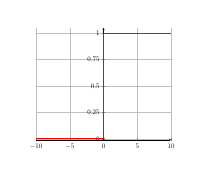
\begin{tikzpicture}[scale=0.25]
            \begin{axis}%
              [ %%%%%%%%%%%%%%%%%
              grid=major, %
              xmin=-10, % 
              xmax=10, % 
              axis x line=bottom, % 
              ytick={0,.25,.5,.75,1.0}, %
              ymax=1.05, % 
              ymin = -0.01, %
              axis y line=middle, % 
              every  axis y label/.style={at={(current axis.north
                  west)},above=2mm} ]% 
              \addplot%
              [ red,line width=0.5mm,%
              mark=none, samples=100, domain=0:10, ]
              (x,{1.00});
              \addplot%
              [ red,line width=0.5mm,%
              mark=none, samples=100, domain=-10:0, ]
              (x,{0.0});
              \addplot%
              [ red,line width=0.5mm,%
              mark=none, samples=100, domain=-10:0]
              (x,{0.0});
              \addplot[ red,line width=0.5mm,%
              mark=none] coordinates {(0,0) (0,1)};%
            \end{axis}
          \end{tikzpicture}\hfill
%%%%%%% logistic
          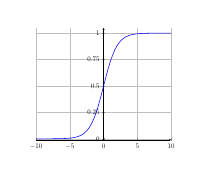
\begin{tikzpicture}[scale=0.25]
            \begin{axis}%
              [ %%%%%%%%%%%%%%%%%
              grid=major, %
              xmin=-10, % 
              xmax=10, % 
              axis x line=bottom, % 
              ytick={0,.25,.5,.75,1.0}, %
              ymax=1.05, % 
              ymin = -0.01, %
              axis y line=middle, % 
              every  axis y label/.style={at={(current axis.north
                  west)},above=2mm} ]% 
              \addplot%
              [ blue,thick,%
              mark=none, samples=100, domain=-10:10, ]
              (x,{1/(1+exp(-x))});
            \end{axis}
          \end{tikzpicture}\hfill
%%%%%%%%% relu
         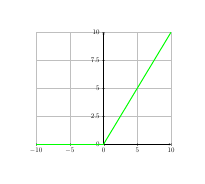
\begin{tikzpicture}[scale=0.25]
            \begin{axis}%
              [ %%%%%%%%%%%%%%%%%
              grid=major, %
              xmin=-10, % 
              xmax=10, % 
              axis x line=bottom, % 
              ytick={0,2.5,5,7.5,10}, %
              ymax=10, % 
              ymin = -0.01, %
              axis y line=middle, % 
              every  axis y label/.style={at={(current axis.north
                  west)},above=2mm} ]% 
              \addplot%
              [ green,line width=0.5mm,%
              mark=none, samples=100, domain=0:-10, ]
              (x,{0.00});
              \addplot%
              [ green,line width=0.5mm,%
              mark=none, samples=100, domain=0:10, ]
              (x,x);
            \end{axis}
          \end{tikzpicture}
  \end{center}
\end{frame}








%%%%%%%%%%%%%%%%%%%%%%%%%%%%%%%%%%%%%%%%%%%%%%%%%%%%%%%%%%%%%%%%%%%%%% 
% - From linear to non-linear classification
% - The feed-forward architecture and the back-propagation algorithm
%%%%%%%%%%%%%%%%%%%%%%%%%%%%%%%%%%%%%%%%%%%%%%%%%%%%%%%%%%%%%%%%%%%%%%
\section{From linear to non-linear classification}
%%%%%%%%%%%%%%%%%%%%%%%%%%%%%%%%%%%%%%%%%%%%%%%%%%%%%%%%%%%%%%%%%%%%%%%%%%%%%%%%%%%%%%%%%
\begin{frame}{Remember: one artificial neuron}
  \framesubtitle{Linear classification and the sigmoid function}
      \begin{columns}
        \column{0.5\textwidth}
        \begin{align*}
      P(\class=1 | \x) &= \sigma(\scal{\vct{w}}{\x}) = y \\
      \sigma(a)  &= \frac{e^a}{1+e^a} = \frac{1}{1+e^{-a}}\\
          a&=\scal{\vct{w}}{\x}, a \in \mathbb{R}\\
          a &=w_0 +  w_1 x_1 + \cdots + w_{\nfeats} x_{\nfeats} \\
          \params &=   (\vct{w}),  \dataset = (\exi, \classi )_{i=1}^n
        \end{align*}
        \column{0.5\textwidth}
        \includegraphics[width=0.9\textwidth]{./figs/reg_log_3d_2.pdf}
  \end{columns}

  \begin{block}{Learning with (Stochastic) Gradient Descent }
    Minimize $\fullloss = \sum_{i=1}^{\nsamples} \ploss(\params,\exi,\classi)$
    $$ \ploss(\params,\exi,\classi) =  - {\color{green!70!black} \underbrace{\classi log(y_{(i)} )}_{\classi=1}}-
    {\color{red!70!black} \underbrace{(1-\classi) log(1-y_{(i)})}_{\classi=0} }$$
  \end{block}
\end{frame}


\begin{frame}{Limits of the linear separation}
  \begin{center}
\includegraphics[width=.45\textwidth]{./figs/linear_1.pdf} 
\includegraphics[width=.45\textwidth]{figs/nonlinear_1.pdf}\\
\includegraphics[width=.45\textwidth]{figs/nonlinear_2.pdf}
\includegraphics[width=.45\textwidth]{figs/many_xor.pdf}
\end{center}
\end{frame}


%%%%%%%%%%%%%%%%%%%%%%%%%%%%%%%%%%%%%%%%%%%%%%%%%%%
\begin{frame}{Case study : X-or}
  \framesubtitle{Starting point}
  \includegraphics[width=.475\textwidth]{figs/many_xor.pdf}
  \includegraphics[width=.475\textwidth]{figs/xor_1/xor_2d.pdf}
  \begin{block}{Hint}
    Try a first linear separation, maybe two. 
  \end{block}
\end{frame}


%%%%%%%%%%%%%%%%%%%%%%%%%%%%%%%%%%%%%%%%%%%%%%%%%%%
\begin{frame}{Case study : X-or}
  \framesubtitle{First try: linear classifiers}
  \vspace{-1cm}
  \begin{flushleft}
    \begin{tikzpicture}
      \node at (0,0)  {\includegraphics[width=.4\textwidth]{figs/xor_1/xor_sep2_2d.pdf}};
      \node at (0,-1.75) {$\vct{w} = [3, -4, -4] $};
      \node at (0.5*\textwidth-8,0)  {\includegraphics[width=.5\textwidth]{figs/xor_1/xor_sep2_3d.pdf}};
  \end{tikzpicture}
\end{flushleft}
\vspace{-1cm}
  \begin{flushleft}
  \begin{tikzpicture}
    \node at (0,0)  {\includegraphics[width=.4\textwidth]{figs/xor_1/xor_sep1_2d.pdf}};
    \node at (0,-1.75) {$\vct{w} = [2.5, 4, 4] $};
    \node at (0.5*\textwidth-8,0)  {\includegraphics[width=.5\textwidth]{figs/xor_1/xor_sep1_3d.pdf}};
  \end{tikzpicture}
\end{flushleft}
\end{frame}


%%%%%%%%%%%%%%%%%%%%%%%%%%%%%%%%%%%%%%%%%%%%%%%%%%%%%%%%%%%%%%%% 
\begin{frame}{A first neural network}
  \framesubtitle{The multi-layer architecture}
  \begin{center}
    \vspace{-1cm}
    \begin{tikzpicture}
      \node[circle,draw ,fill=gray!20, minimum size=3ex,inner sep=0pt]  (x1) at (0,0) {\small $x_1$};% in 1
      \node[circle,draw ,fill=gray!20, minimum size=3ex,inner sep=0pt]  (x2) at (0,1) {\small $x_2$};% in 2
      \node[circle,draw ,fill=gray!60, minimum size=3ex,inner sep=0pt]  (b1) at (0,2) {\small $1$};% b1 1
      %%%% 
      \uncover<2->{
        \node[circle,draw, minimum size=3ex,inner sep=0pt]  (z1) at (2,1) {\small $z_1$};% h 1
      \draw[->-] (x1) -- (z1) ;
      \draw[->-] (x2) -- (z1) ;
      \draw[->-] (b1) -- (z1) ;
      \node at (3,1.5) {\includegraphics[width=0.15\textwidth]{{figs/xor_1/xor_sep1_3d.pdf}}};
      }
      %%%% 
      \uncover<3->{
        \node[circle,draw, minimum size=3ex,inner sep=0pt]  (z2) at (2,0) {\small $z_2$};% h 2
        \draw[->-] (x1) -- (z2) ;
        \draw[->-] (x2) -- (z2) ;
        \draw[->-] (b1) -- (z2) ;      
        \node at (3,-0.5) {\includegraphics[width=0.15\textwidth]{{figs/xor_1/xor_sep2_3d.pdf}}};
      }
      %%%%%
      \uncover<4->{
        \node[circle,draw, minimum size=3ex,inner sep=0pt]  (y) at (4,1) {\small $y$};% out
        \node[circle,draw ,fill=gray!60, minimum size=3ex,inner sep=0pt]  (b2) at (2,2) {\small $1$};% b1 1        
        \draw[->-] (z1) -- (y) ;
        \draw[->-] (z2) -- (y) ;
        \draw[->-] (b2) -- (y) ;
        \node (out) at (8,1) {\includegraphics[width=0.6\textwidth]{{figs/xor_1/xor_mlp_3d.pdf}}};
        \draw[->] (4.5,1) -- (6,1);
      }
      \uncover<5->{
        \node[draw=blue,ultra thick,fit=(x1) (x2) (b1)] {} ;
        \node[draw=blue,ultra thick,fit=(z1) (z2) (b2)] {} ;
%        \node[fill=blue!20,rectangle] at (1,1)  {$\mathbf{W_1}$};
      }        
    \end{tikzpicture}
  \end{center}

  \uncover<5->{
    \vspace{-4ex}
    \begin{itemize}
    \item The network is organized by layers: input ($\vct{x}$), hidden  ($\vct{z}$), and output  ($\vct{y}$)
    \item Two layers are fully connected % : A matrix gathers the connection weights: $\mathbf{W_1}$
    \item The propagation of the input is sequential: 
    \end{itemize}
    \begin{align*}
      z_1 &= f(\scal{\seq{v}_1}{\x}) \textrm{ and }  z_2 = f(\scal{\seq{v}_2}{\x})) &\Rightarrow \seq{z} = f(\seq{V}\x)\\
      y &= f(\scal{\seq{w}}{\seq{z}}) &\Rightarrow y = f(\seq{W}\seq{z})\\
    \end{align*}
    % $$
    % \vct{x} \rightarrow \vct{z} \rightarrow \vct{y}
    % $$
    % $$
    % \vct{z} = f(\vct{W_1}\vct{x})
    % $$
    }
  \end{frame}



  
  \begin{frame}{Another view of the neural network}
%    \framesubtitle{Learning a new representation of the data}
    \framesubtitle{Representation learning}
    \begin{center}
       \begin{tikzpicture}[scale=0.6]
      \node[circle,draw ,fill=gray!20, minimum size=3ex,inner sep=0pt]  (x1) at (0,0) {\small $x_1$};% in 1
      \node[circle,draw ,fill=gray!20, minimum size=3ex,inner sep=0pt]  (x2) at (0,1) {\small $x_2$};% in 2
      \node[circle,draw ,fill=gray!60, minimum size=3ex,inner sep=0pt]  (b1) at (0,2) {\small $1$};% b1 1
      %%%% 
      \node[circle,draw, minimum size=3ex,inner sep=0pt]  (z1) at (3,1) {\small $z_1$};% h 1
      \draw[->-] (x1) -- (z1) ;
      \draw[->-] (x2) -- (z1) ;
      \draw[->-] (b1) -- (z1) ;
      %%%% 
      \node[circle,draw, minimum size=3ex,inner sep=0pt]  (z2) at (3,0) {\small $z_2$};% h 2
      \draw[->-] (x1) -- (z2) ;
      \draw[->-] (x2) -- (z2) ;
      \draw[->-] (b1) -- (z2) ;      
      %%%%% 
      \node[circle,draw, minimum size=3ex,inner sep=0pt]  (y) at (6,1) {\small $y$};% out
      \node[circle,draw ,fill=gray!60, minimum size=3ex,inner sep=0pt]  (b2) at (3,2) {\small $1$};% b1 1        
      \draw[->-] (z1) -- (y) ;
      \draw[->-] (z2) -- (y) ;
      \draw[->-] (b2) -- (y) ;
      \node[draw=blue,ultra thick,fit=(x1) (x2) (b1)] {} ;
      \node[draw=blue,ultra thick,fit=(z1) (z2) (b2)] {} ;
      \node[draw=blue,ultra thick,fit=(y)] {} ;
      \node[fill=blue!20,rectangle] at (1.5,1)  {$\seq{V}$};
      \node[fill=blue!20,rectangle] at (4.5,1)  {$\seq{W}$};
      \end{tikzpicture}
      \begin{tikzpicture}
        \node at (-1.5,-2) {\includegraphics[width=.4\textwidth]{figs/many_xor.pdf}};
        \node at (3.5,-2) {\includegraphics[width=.4\textwidth]{figs/many_xor_projected.pdf}};
      \end{tikzpicture}
    \end{center}
    \vspace{-4ex}
    \begin{itemize}
    \item The network learns its own representation $\seq{z}$. 
    \item The final decision is linear.
    \end{itemize}
\end{frame}

% xor 


\begin{frame}{Summary}
  \framesubtitle{The multi-layer or feed-forward architecture}
    \begin{columns}
      %%%%%%%%%%%%% Column 1 
      \column{0.6\textwidth}
      \begin{itemize}
      \item 1 neuron = 1 value;  1 layer = 1 vector 
      \item Two layers ($\seq{x}, \seq{z}$)  fully connected: $$ \seq{z} = f(\seq{V} \seq{x})$$
      \item Inference: a sequential propagation %  (matrix operation)
      \item Hidden layer ($\seq{z})$: the internal representation  
      \end{itemize}
      %%%%%%%%%%%%% Column 2 
      \column{0.4\textwidth}
      \begin{tikzpicture}[scale=0.6]
        \node[circle,draw ,fill=gray!20, minimum size=3ex,inner sep=0pt]  (x1) at (0,0) {\small $x_1$};% in 1
        \node[circle,draw ,fill=gray!20, minimum size=3ex,inner sep=0pt]  (x2) at (0,1) {\small $x_2$};% in 2
        \node[circle,draw ,fill=gray!60, minimum size=3ex,inner sep=0pt]  (b1) at (0,2) {\small $1$};% b1 1
        %%%% 
        \node[circle,draw, minimum size=3ex,inner sep=0pt]  (z1) at (3,1) {\small $z_1$};% h 1
        \draw[->-] (x1) -- (z1) ;
        \draw[->-] (x2) -- (z1) ;
        \draw[->-] (b1) -- (z1) ;
        %%%% 
        \node[circle,draw, minimum size=3ex,inner sep=0pt]  (z2) at (3,0) {\small $z_2$};% h 2
        \draw[->-] (x1) -- (z2) ;
        \draw[->-] (x2) -- (z2) ;
        \draw[->-] (b1) -- (z2) ;      
        %%%%% 
        \node[circle,draw, minimum size=3ex,inner sep=0pt]  (y) at (6,1) {\small $y$};% out
        \node[circle,draw ,fill=gray!60, minimum size=3ex,inner sep=0pt]  (b2) at (3,2) {\small $1$};% b1 1        
        \draw[->-] (z1) -- (y) ;
        \draw[->-] (z2) -- (y) ;
        \draw[->-] (b2) -- (y) ;
        \node[draw=blue,ultra thick,fit=(x1) (x2) (b1)] {} ;
        \node[draw=blue,ultra thick,fit=(z1) (z2) (b2)] {} ;
        \node[draw=blue,ultra thick,fit=(y)] {} ;
        \node[fill=blue!20,rectangle] at (1.5,1)  {$\seq{V}$};
        \node[fill=blue!20,rectangle] at (4.5,1)  {$\seq{W}$};
      \end{tikzpicture}
  \end{columns}
\end{frame}




\begin{frame}{Exercise: the X-or network}
  \begin{center}
    \vspace{-1cm}
    \begin{tikzpicture}
      \node[circle,draw ,fill=gray!20, minimum size=3ex,inner sep=0pt]  (x1) at (0,0) {\small $x_1$};% in 1
      \node[circle,draw ,fill=gray!20, minimum size=3ex,inner sep=0pt]  (x2) at (0,1) {\small $x_2$};% in 2
      \node[circle,draw ,fill=gray!60, minimum size=3ex,inner sep=0pt]  (b1) at (0,2) {\small $1$};% b1 1
      %%%% 
        \node[circle,draw, minimum size=3ex,inner sep=0pt]  (z1) at (2,1) {\small $z_1$};% h 1
      \draw[->-] (x1) -- (z1) ;
      \draw[->-] (x2) -- (z1) ;
      \draw[->-] (b1) -- (z1) ;
      \node at (3,1.5) {\includegraphics[width=0.15\textwidth]{{figs/xor_1/xor_sep1_3d.pdf}}};
      %%%% 
        \node[circle,draw, minimum size=3ex,inner sep=0pt]  (z2) at (2,0) {\small $z_2$};% h 2
        \draw[->-] (x1) -- (z2) ;
        \draw[->-] (x2) -- (z2) ;
        \draw[->-] (b1) -- (z2) ;      
        \node at (3,-0.5) {\includegraphics[width=0.15\textwidth]{{figs/xor_1/xor_sep2_3d.pdf}}};
      %%%%%
        \node[circle,draw, minimum size=3ex,inner sep=0pt]  (y) at (4,1) {\small $y$};% out
        \node[circle,draw ,fill=gray!60, minimum size=3ex,inner sep=0pt]  (b2) at (2,2) {\small $1$};% b1 1        
        \draw[->-] (z1) -- (y) ;
        \draw[->-] (z2) -- (y) ;
        \draw[->-] (b2) -- (y) ;
        \node (out) at (8,1) {\includegraphics[width=0.6\textwidth]{{figs/xor_1/xor_mlp_3d.pdf}}};
        \draw[->] (4.5,1) -- (6,1);
        \node[draw=blue,ultra thick,fit=(x1) (x2) (b1)] {} ;
        \node[draw=blue,ultra thick,fit=(z1) (z2) (b2)] {} ;
%        \node[fill=blue!20,rectangle] at (1,1)  {$\mathbf{W_1}$};
    \end{tikzpicture}
    Compute the parameters of the output neuron  ($\seq{W}$) ? \\
    What is its activation function ?
  \end{center}
\end{frame}

\newcommand{\cone}{\color{green!30!black}}
\newcommand{\czero}{\color{red!30!black}}
\begin{frame}{Exercise : the X-or problem}
  From a boolean algebra point of view. Assume {\cone true value is 1} and {\czero false is 0}
  %%%%%%%%%%%%%%%%
  \begin{columns}
    \column{0.3\textwidth}
    \begin{center}
      \includegraphics[width=\textwidth]{figs/xor_1/xor_sep1_2d.pdf}
    \end{center}
    %%%%
    \column{0.7\textwidth}
    \begin{itemize}
    \item Write the truth table. 
    \item Provide an interpretation as a boolean operator
    \end{itemize}    
  \end{columns}
  %%%%%%%%%%%%%%%%
  \begin{columns}
    \column{0.3\textwidth}
    \begin{center}
      \includegraphics[width=\textwidth]{figs/xor_1/xor_sep2_2d.pdf}
    \end{center}
    %%%%
    \column{0.7\textwidth}
        \begin{itemize}
        \item  Write the truth table. 
        \item Provide an interpretation as a boolean operator
    \end{itemize}    
  \end{columns}
  Write the boolean operation implemented by the previous neural network by merging the two previsous steps. 
\end{frame}

%%%%%%%%%%%%%%%%%%%%%%%%%%%%%%%%%%%%%%%%%%%%%%%%%%%%%%%%%%%%%%%%%%%%%%
% - Back propagation on a simple case 
%%%%%%%%%%%%%%%%%%%%%%%%%%%%%%%%%%%%%%%%%%%%%%%%%%%%%%%%%%%%%%%%%%%%%%
\section{Multi-layered neural network and the back-propagation algorithm}

%%%%%%%%%%%%%%%%%%%%%%%%%%%%%%%%%%%%%%%%%%%%%%%%%%%%%%%%%%
%
% WARNING : use common_nnet.tex
% Alex. Allauzen, 18 jan. 2020
%%%%%%%%%%%%%%%%%%%%%%%%%%%%%%%%%%%%%%%%%%%%%%%%%%%%%%%%%%
\begin{frame}{For a shallow network, with a single layer}
  \begin{columns}
    \begin{column}{0.5\textwidth}
    \begin{center}
      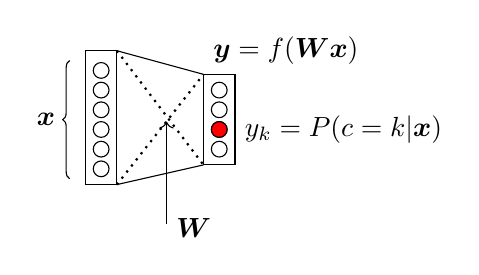
\begin{tikzpicture}
        \begin{scope}
          % input
          \node (nx) at (-0.7,0.625){$\x$}; %
          \foreach \y in {0,0.25,...,1.25}{ \draw (0,\y) circle
            (0.1cm);%
          } \draw (-0.2,-0.2) rectangle (0.2,1.5); \draw[snake=brace]
          (-0.4,-0.125) -- (-0.4,1.375);
          % output
          \foreach \y in {0.25,0.5,...,1}{ \draw (1.5,\y) circle
            (0.1cm);%
          } \draw (1.3,0.05) rectangle (1.7,1.2); \draw (0.2,-0.2) --
          (1.3,0.05); % high link between layers
          \draw (0.2,1.5) -- (1.3,1.2);% low link between layers
          \draw[dotted, thick] (0.2,1.5) -- (1.3,0.05);
          \draw[dotted,thick] (0.2,-0.2) -- (1.3,1.2);
          % \draw[snake=brace] ( 1.8, 1.2) --(1.8, 0.05) ;
          \node[anchor=west] (ny) at
          (1.3,1.5){$\outp=f(\W \x)$}; %
          \node[anchor=west] (nW) at (0.83,-0.75){$\W$};%
          \draw[->] (0.83,-0.7) -- (0.83,0.6);%
          % fill one output unit
          \draw[fill=red] (1.5,0.5) circle (0.1cm);
          \node[anchor=west] (nyk) at (1.7,0.5){$y_k =
            P(c=k|\x)$};%
        \end{scope}
      \end{tikzpicture}
    \end{center}
  \end{column}
  %%% matrix view
  \begin{column}{0.5\textwidth}
     $$
     \params = (\W)
     $$
  \end{column}
  \end{columns}
  %%%%%%%%%%%
  \begin{center}
  $$
  \begin{array}{ll|ll}
    \multicolumn{2}{c|}{\textrm{Forward (inference)}} &    \multicolumn{2}{c}{\textrm{Backward (gradient)}} \\\hline
    &&&\\
    %%% l1 
    \ploss(\params,\exi,\classi) &\leftarrow \outp
    &\displaystyle \frac{\partial \ploss(\params,\exi,\classi) }{\partial\W}= &\displaystyle \frac{\partial \ploss(\params,\exi,\classi) }{\partial\outp} \\[1.5ex]
    %%% l2
    \outp &= f(\seq{a})
    & &\displaystyle \times \frac{\partial \outp }{\partial\seq{a}} \\[1.5ex]
    %%% l3
    \seq{a} &= \W\inp
    &  &\displaystyle \times \frac{\partial \seq{a} }{\partial\W} 
  \end{array}
  $$
\end{center}
\end{frame}




\begin{frame}{Review of the gradient computation}
  \framesubtitle{Without hidden layer (shallow net)}
  \setlength{\tabcolsep}{1pt} % less space between columns in tabular (default is 6pt
  $\ploss$ is the shortcut for $\ploss(\classi, \x\sid{i}, \params\tid{i})$ 
  \begin{center}
  \begin{tabular}{ccccccc}
    \tikz[baseline]{\node[anchor=base] (grad) 
    {$\frac{\partial \ploss}{\partial \W}$};}
    &=
    &\tikz[baseline]{\node[fill=red!20,anchor=base] (loss) 
      {$\frac{\partial \ploss}{\partial \yi} $};}
    &$\times$  
    &\tikz[baseline]{\node[fill=red!20,anchor=base] (outp) 
      {$\frac{\partial  \yi  }{\partial \pa}$};}
    &$\times$
    &\tikz[baseline]{\node[fill=green!20,anchor=base] (inp) 
      {$ \frac{\partial \pa}{\partial \W}$};}\\[6ex] %%%%%%%
    \tikz[baseline]{\node[anchor=base] (grad2){Supervision};}
    &
    &\tikz[baseline]{\node[anchor=base,rounded corners,fill=red!20] (loss2){\small loss \textit{vs} output};}
    &
    &\tikz[baseline]{\node[anchor=base,rounded corners,fill=red!20] (outp2){\small activation};}
    &
    &\tikz[baseline]{\node[anchor=base,rounded corners,fill=green!20] (inp2){ \small gradient of $\W$};}\\[6ex]
    & &\multicolumn{3}{c}{\tikz[baseline]{\node[anchor=base,rounded corners,fill=red!20] (err){
        \small
        \begin{tabular}{c}
          Error signal \\ from supervision\\and output
        \end{tabular}
    };}}
    &
    & \tikz[baseline]{\node[anchor=base,rounded corners,fill=green!20] (inp3){
      \small\begin{tabular}{c}
              Contribution \\of $\W$\\
              $\rightarrow \x$
            \end{tabular}};}
  \end{tabular}
\end{center}


  \begin{tikzpicture}[overlay]
    \path[->](grad) edge  (grad2);
    \path[->](loss) edge  (loss2);
    \path[->](outp) edge  (outp2);
    \path[->](inp) edge  (inp2);
    \path[->](loss2) edge  (err);
    \path[->](outp2) edge  (err);
    \path[->](inp2) edge  (inp3);
  \end{tikzpicture}
\end{frame}



\begin{frame}{In the matrix form}
  \begin{center}
  \begin{tabular}{ccccc}
    \tikz[baseline]{\node[anchor=base] (grad) 
    {$\pgrad{\W} = \frac{\partial \ploss}{\partial \W}$};}
    &=
    &\tikz[baseline]{\node[fill=red!20,anchor=base] (l) 
      {$\frac{\partial \ploss}{\partial \yi} \times \frac{\partial  \yi  }{\partial \pa} $};}
    &$\times$  
    &\tikz[baseline]{\node[fill=green!20,anchor=base] (i) 
      {$ \frac{\partial \pa}{\partial \W}$};}\\[6ex]
    %%%%%%%%%%%%%%%%%%%%%%%%%
    &=
    &\tikz[baseline]{\node[fill=red!20,anchor=base] (l2) 
      {$\vdlta_{\W}$};}
    &$\times$  
    &\tikz[baseline]{\node[fill=green!20,anchor=base] (i2) 
      {$ \x^{t}$};}\\[6ex]
    %%%%%%%%%%%%%%%%%%%%%%%%%
    &= 
    &\tikz[baseline]{\node[fill=red!20,anchor=base] (l3) 
      {$(\nclasses,1) $};}
    &$\times$  
    &\tikz[baseline]{\node[fill=green!20,anchor=base] (i3)
      {$(1,\nfeats) $};}\\[6ex]
    %%%%%%%%%%%%%%%%%%%%%%%%% 
    &$=$
    &\tikz[baseline]{\node[anchor=base,rounded corners,fill=red!20] (l4){\small
      \begin{tabular}{c}
        Gradient \\up to the \\pre-activation
      \end{tabular}
      };}
    &$\times$  
    &\tikz[baseline]{\node[anchor=base,rounded corners,fill=green!20] (i4){\small
      \begin{tabular}{c}
        input of\\the layer
      \end{tabular}
      };}
  \end{tabular}
\end{center}

\begin{tikzpicture}[overlay]
  \path[->](l) edge  (l2);
  \path[->](i) edge  (i2);
  \path[->](l2) edge  (l3);
  \path[->](i2) edge  (i3);
  \path[->](l3) edge  (l4);
  \path[->](i3) edge  (i4);
\end{tikzpicture}

\begin{itemize}
\item $\pgrad{\W}$ is a matrix of size $(\nclasses,\nfeats)$
\item $\pgrad{\W}[i,j] = \vdlta[i] \times \x[j]$
\end{itemize}
  
\end{frame}

\begin{frame}{Gradient computation with one hidden layer}
  \begin{columns}
    %%%%%%%%%%%%% Column 1
    \column{0.5\textwidth}
    \begin{center}
    \begin{tikzpicture}[scale=0.6]
      \node[circle,draw ,fill=gray!20, minimum size=3ex,inner sep=0pt]  (x1) at (0,0) {\small $x_1$};% in 1
      \node[circle,draw ,fill=gray!20, minimum size=3ex,inner sep=0pt]  (x2) at (0,1) {\small $x_2$};% in 2
      \node[circle,draw ,fill=gray!60, minimum size=3ex,inner sep=0pt]  (b1) at (0,2) {\small $1$};% b1 1
      %%%% 
      \node[circle,draw, minimum size=3ex,inner sep=0pt]  (z1) at (3,1) {\small $z_1$};% h 1
      \draw[->-] (x1) -- (z1) ;
      \draw[->-] (x2) -- (z1) ;
      \draw[->-] (b1) -- (z1) ;
      %%%% 
      \node[circle,draw, minimum size=3ex,inner sep=0pt]  (z2) at (3,0) {\small $z_2$};% h 2
      \draw[->-] (x1) -- (z2) ;
      \draw[->-] (x2) -- (z2) ;
      \draw[->-] (b1) -- (z2) ;      
      %%%%% 
      \node[circle,draw, minimum size=3ex,inner sep=0pt]  (y) at (6,1) {\small $y$};% out
      \node[circle,draw ,fill=gray!60, minimum size=3ex,inner sep=0pt]  (b2) at (3,2) {\small $1$};% b1 1        
      \draw[->-] (z1) -- (y) ;
      \draw[->-] (z2) -- (y) ;
      \draw[->-] (b2) -- (y) ;
      \node[draw=blue,ultra thick,fit=(x1) (x2) (b1)] {} ;
      \node[draw=blue,ultra thick,fit=(z1) (z2) (b2)] {} ;
      \node[draw=blue,ultra thick,fit=(y)] {} ;
      \node[fill=blue!20,rectangle] at (1.5,1)  {$\seq{V}$};
      \node[fill=blue!20,rectangle] at (4.5,1)  {$\seq{W}$};
    \end{tikzpicture}
  \end{center}
    %%%%%%%%%%%%% Column 1 
    \column{0.5\textwidth}
    Two questions (or gradients): 
    {\large
      \begin{itemize}
      \item $\frac{\partial \ploss}{\partial \W} =~ ? $
      \item $\frac{\partial \ploss}{\partial \V} =~ ? $
      \end{itemize}
    }
  \end{columns}
\end{frame}



\begin{frame}{Gradient computation with one hidden layer}
  \framesubtitle{Step 1: $\W$}
  \begin{center}
    \begin{tabular}{ccccccc}
      \tikz[baseline]{\node[anchor=base] (grad) 
      {$\frac{\partial \ploss}{\partial \W}$};}
      &=
      &\tikz[baseline]{\node[fill=red!20,anchor=base] (loss) 
        {$\frac{\partial \ploss}{\partial \yi} $};}
      &$\times$  
      &\tikz[baseline]{\node[fill=red!20,anchor=base] (outp) 
        {$\frac{\partial  \yi  }{\partial \pa}$};}
      &$\times$
      &\tikz[baseline]{\node[fill=blue!20,anchor=base] (inp) 
        {$ \frac{\partial \pa}{\partial \W}$};}\\[6ex] %%%%%%%
      \tikz[baseline]{\node[anchor=base] (grad2){Supervision};}
      &
      &\tikz[baseline]{\node[anchor=base,rounded corners,fill=red!20] (loss2){\small loss \textit{vs} output};}
      &
      &\tikz[baseline]{\node[anchor=base,rounded corners,fill=red!20] (outp2){\small activation};}
      &
      &\tikz[baseline]{\node[anchor=base,rounded corners,fill=blue!20] (inp2){ \small gradient of $\W$};}\\[6ex]
      & &\multicolumn{3}{c}{\tikz[baseline]{\node[anchor=base,rounded corners,fill=red!20] (err){
          \small $\vdlta_{\W}$};}}
      &$\times$
      & \tikz[baseline]{\node[anchor=base,rounded corners,fill=blue!20] (inp3){
        \small$\z^t$};}
    \end{tabular}
  \end{center}
  \begin{tikzpicture}[overlay]
    \path[->](grad) edge  (grad2);
    \path[->](loss) edge  (loss2);
    \path[->](outp) edge  (outp2);
    \path[->](inp) edge  (inp2);
    \path[->](loss2) edge  (err);
    \path[->](outp2) edge  (err);
    \path[->](inp2) edge  (inp3);
  \end{tikzpicture}
  \begin{itemize}
  \item Very similar to the shallow network, but the ``input'' is $\z$ instead of $\x$  
  \item But $\z$ is computed by the network (parameters $\V$)
  \end{itemize}
\end{frame}

\begin{frame}{Gradient computation with one hidden layer}
  \framesubtitle{Step 2 : $\V$}
  Denote the pre-activation of the input layer $\pb = \V\x$
    \begin{center}
    \begin{tabular}{ccccccc}
      \tikz[baseline]{\node[anchor=base] (grad) 
      {$\frac{\partial \ploss}{\partial \V}$};}
      &=
      &\tikz[baseline]{\node[fill=red!20,anchor=base] (loss) 
        {$\frac{\partial \ploss}{\partial \yi}\times\frac{\partial  \yi  }{\partial \pa} $};}
      &$\times$  
      &\tikz[baseline]{\node[fill=blue!20,anchor=base] (inner) 
        {$\frac{\partial  \pa  }{\partial \z}\times\frac{\partial  \z  }{\partial \pb}$};}
      &$\times$
      &\tikz[baseline]{\node[fill=green!20,anchor=base] (inp) 
        {$ \frac{\partial \pb}{\partial \V}$};}\\[6ex] %%%%%%%
      &
      & \tikz[baseline]{\node[anchor=base,rounded corners,fill=red!20] (err){$\vdlta_{W}$  };}
      &
      & \tikz[baseline]{\node[anchor=base,rounded corners,fill=blue!20] (inner2){
          \footnotesize
          \begin{tabular}{c}
            Through $\W$\\ and \\  the activation
          \end{tabular}
      };}
      &
      &  \tikz[baseline]{\node[anchor=base,rounded corners,fill=green!20] (inp2){
        \footnotesize\begin{tabular}{c}
                Contribution \\of $\V$\\
                 $\rightarrow\x$
              \end{tabular}};}
    \end{tabular}
  \end{center}
    \begin{tikzpicture}[overlay]
    \path[->](loss) edge  (err);
    \path[->](inner) edge  (inner2);
    \path[->](inp) edge  (inp2);
    \path[->](err) edge  (inner2);
    \path[->](inner2) edge  (inp2);
  \end{tikzpicture}
  \begin{itemize}
  \item The error signal $\vdlta_{W}$ is back-propagated through $\W$, 
  \item to get $\vdlta_{V}$
  \item The update for $\V$ is $\pgrad{\V} = \vdlta_{V}\z^t$
  \end{itemize}
\end{frame}

\begin{frame}{The back-propagation algorithm for a feed-forward network with one hidden layer}
  \framesubtitle{Introduced in \cite{Rumelhart86BP}}
  One iteration of the online version, for a given value of $\params$:
  \begin{enumerate}
  \item Foward propagation of $\exi$ ($\rightarrow\ \z$ and $\y\sid{i}$)
  \item Compute the loss 
  \item Back-propagation and collect of  the gradients:
    \begin{itemize}
    \item output layer: $\vdlta_{W}$ and $\pgrad{\W} = \vdlta_{W}\z^t$
    \item input layer: $\vdlta_{V}$ and $\pgrad{\V} = \vdlta_{V}\x^t$
    \end{itemize}
  \item Update parameters:
    \begin{align*}
      \W &= \W - \eta \pgrad{\W} \\
      \V &= \V - \eta \pgrad{\V} 
    \end{align*}
  \end{enumerate}
\end{frame}


%%%%%%%%%%%%%%%%%%%%%%%%%%%%%%%%%%%%%%%%%%%%%%%%%%%%%%%%%%%%%%%%%%%%%%%%%%%%%%%%%%%%%%%%%%%%%%%%%%%
%%%%%%%%%%%%%%%%%%%%%%%%%%%%%%%%%%%%%%%%%%%%%%%%%%%%%%%%%%%%%%%%%%%%%%%%%%%%%%%%%%%%%%%%%%%%%%%%%%%
%% Multi-layers
%%%%%%%%%%%%%%%%%%%%%%%%%%%%%%%%%%%%%%%%%%%%%%%%%%%%%%%%%%%%%%%%%%%%%%%%%%%%%%%%%%%%%%%%%%%%%%%%%%%
%%%%%%%%%%%%%%%%%%%%%%%%%%%%%%%%%%%%%%%%%%%%%%%%%%%%%%%%%%%%%%%%%%%%%%%%%%%%%%%%%%%%%%%%%%%%%%%%%%%
\begin{frame}{Notations for a multi-layer neural network (feed-forward)}
  \begin{block}{One layer, indexed by $l$}
    \begin{columns}
      \begin{column}{0.3\textwidth}
        \begin{tabular}[h]{lcl}
          \inp\lid{l} & & \\
          \layer &\connection &\layer\\[-2ex]
          & \raisebox{\raiseW}{\W\lid{l}} &\outp\lid{l} 
        \end{tabular} 
      \end{column}
      \begin{column}{0.7\textwidth}
        \begin{itemize}
        \item \inp\lid{l}: input of the layer $l$
        \item \outp\lid{l} =  $f$\lid{l}(\W\lid{l} \inp\lid{l})
        \item stacking layers:  \outp\lid{l} $=$ \inp\lid{l+1} 
        \item \inp\lid{1}  = a data example
        \end{itemize}
      \end{column}
    \end{columns}
  \end{block}
  
  \vspace{-2ex}
  \begin{center}
    \begin{tabular}[h]{lclclclclcl}
      \color{red}\inp\lid{1} & & \inp\lid{2}  && \inp\lid{3} & &\inp\lid{L} \\
      \color{red}\layer &\connection &\layer &\connection &\layer &\dotted &\layer &\connection &\color{red}\layer \\[-2ex]
      & \raisebox{\raiseW}{\W\lid{1}} &\outp\lid{1}   &\raisebox{\raiseW}{\W\lid{2}} &\outp\lid{2}  &&\outp\lid{L-1}&\raisebox{\raiseW}{\W\lid{L}} &\color{red}\outp\lid{L}: output 
    \end{tabular}
  \end{center}
\end{frame}


%%%%%%%%%%%%%%%%%%%%%%%%%%%%%%%%%%%%%%%%%%%%%%%%%%%%%%%%%%%%%%%%%%%%%%%%%%%%%%%%%%%%%%%%%%%%%%%%%%%
% with one hidden layer  : x is no more x but x2 = y1 = W1 x1 = W1 x
% We can update W2 but what about W1 ? 
%%%%%%%%%%%%%%%%%%%%%%%%%%%%%%%%%%%%%%%%%%%%%%%%%%%%%%%%%%%%%%%%%%%%%%%%%%%%%%%%%%%%%%%%%%%%%%%%%%%
\begin{frame}{Example : with one hidden layer}
  \begin{columns}
    \begin{column}{0.7\textwidth}
      \begin{center}
        \begin{tabular}[h]{lclclr}
          \color{red}\inp\lid{1} & & \inp\lid{2}  && \\
          \color{red}\layer &\connection &\layer &\connection &\layer \\[-2ex]
          & \raisebox{\raiseW}{\W\lid{1}} &\outp\lid{1}   &\raisebox{\raiseW}{\W\lid{2}} &\color{red}\outp\lid{2}: output 
        \end{tabular}
      \end{center}
     \end{column}
    \begin{column}{0.3\textwidth}
      $\params=(\W\lid{1},\W\lid{2})$
    \end{column}
  \end{columns}
  \begin{block}{To learn, we need the gradients for: }
    \begin{itemize}
    \item the output layer: $\pgrad{\W\lid{2}}$
    \item the hidden layer: $\pgrad{\W\lid{1}}$
    \end{itemize}
  \end{block}
\end{frame}


%%%%%%%%%%%%%%%%%%%%%%%%%%%%%%%%%%%%%%%%%
\begin{frame}{Back-propagation: generalization}
  For a hidden layer $l$:
  \begin{itemize}
  \item  The gradient at the pre-activation level: 
    $$
    \vdlta\lid{l} = {f'}\lid{l}(\seq{a}\lid{l})\circ \big({\W\lid{l+1}}^t \vdlta\lid{l+1}\big)
    $$
  \item The update is as follows: 
    $$
    \W\lid{l} =     \W\lid{l}  - \eta_t  \vdlta\lid{l}{\x\lid{l}}^t
    $$
  \end{itemize}
  The layer should keep: 
  \begin{itemize}
  \item $\W\lid{l}$: the parameters
  \item $f\lid{l}$: its activation function
  \item $\inp\lid{l}$: its input
  \item $\seq{a}\lid{l}$: its pre-activation associated to the input
  \item $\vdlta\lid{l}$: for the update and the back-propagation to the layer $l-1$
  \end{itemize}
\end{frame}


\begin{frame}{Back-propagation: one training step}
Pick a training example: $\inp\lid{1} = \x\sid{i}$
  \begin{block}{Forward pass}
    For $l=1$ to $(L-1)$
    \begin{itemize}
    \item Compute $\outp\lid{l}=f\lid{l}(\W\lid{l}\inp\lid{l})$
    \item $\inp\lid{l+1} = \outp\lid{l}$
    \end{itemize}
    $\outp\lid{L}=f\lid{L}(\W\lid{L}\inp\lid{L})$
  \end{block}
  \begin{block}{Backward pass}
    % $$\vdlta\lid{L} = \frac{\partial
    %   \ploss(\params,\exi,\classi)}{\partial \seq{a}\lid{L}}$$
    Init: $\vdlta\lid{L} = \pgrad{\seq{a}\lid{L}}$\\
    For $l=L$ to $2$ {\color{gray!80}// all hidden units}
    \begin{itemize}
    \item $\vdlta\lid{l-1} = {f'}\lid{l-1}(\seq{a}\lid{l-1})\circ \big({\W\lid{l}}^t \vdlta\lid{l}\big)$
    \item $\W\lid{l} = \W\lid{l}  - \eta_t  \vdlta\lid{l}{\x\lid{l}}^t$
    \end{itemize}
    $\W\lid{1} = \W\lid{1}  - \eta_t  \vdlta\lid{1}{\x\lid{1}}^t$
  \end{block}
\end{frame}



\begin{frame}{Conclusion on back-propagation for one layer $l$}
  Training a NNet relies on forward-backward propagation. 
  \begin{block}{Forward:}
    \begin{itemize}
    \item get $\inp\lid{l}$ for the previous layer;
    \item compute and send $\outp\lid{l}=f\lid{l}(\W\lid{l}\inp\lid{l})$.
    \end{itemize}
  \end{block}
  \begin{block}{Backward:}
    \begin{itemize}
    \item get $\vdlta\lid{l}$ as input from the up-comming
      layer;
    \item compute and send $\vdlta\lid{l-1}$ to the previous layer;
    \item update parameters $\W\lid{l}$
    \end{itemize}
  \end{block}
\end{frame}


\begin{frame}{Initialization recipes}
  A difficult question with several empirical answers. 
  \begin{block}{One standard trick}
    $$\W \sim \mathcal{N}(0,\frac{1}{\sqrt{n_{in}}})  $$
    with $n_{in}$ is the number of inputs
  \end{block}
  \begin{block}{A more recent one}
    $$\W \sim \mathcal{U}
    \Big[-\frac{\sqrt{6}}{\sqrt{n_{in}+n_{out}}},
    \frac{\sqrt{6}}{\sqrt{n_{in}+n_{out}}} \Big]  $$
    with $n_{in}$ is the number of inputs
  \end{block}
\end{frame}





\section{Summary}
\begin{frame}
  \frametitle{Summary}
  \begin{block}{Multi-layered Perceptron (MLP) or feed-forward NNet}
    \begin{itemize}
    \item Artificial neurons are organizes in \important{layers}:  $\rightarrow$ a vector  
    \item Two layers are in general \important{fully connected}
      \begin{itemize}
      \item A linear transformation parametrized by a matrix
      \item followed  by a pointwise non-linear function, the
        activation function
      \end{itemize}
    \item A \important{feed-forward} architecture is a stack of layers
      fully connected 
    \item[$\rightarrow$] Can approximate any functions depending on the number of hidden
      units. 
    \end{itemize}
  \end{block}
  \begin{block}{Training by back-propagation}
    \begin{itemize}
    \item After a forward pass (inference from input to the output) 
    \item Backward pass (compute the gradients of each layer from the
      output to the input)
    \end{itemize}
  \end{block}
\end{frame}


%%%%%%%%%%%%%%%%%%%%%%%%%%%%%%%%%%%%%%%%%%%%%%%%
\bibliographystyle{../styles/naaclhlt2012}
{\footnotesize \bibliography{./alex}}
%%%%%%%%%%%%%%%%%%%%%%%%%%%%%%%%%%%%%%%%%%%%%%%%
\end{document}
